% Character tables of S3, S4 and A5, each cell coloured by the value divided by the dimension (orange positive, blue negative). Rows: irreducible characters; columns: conjugacy classes with their sizes. Generated by a short script.
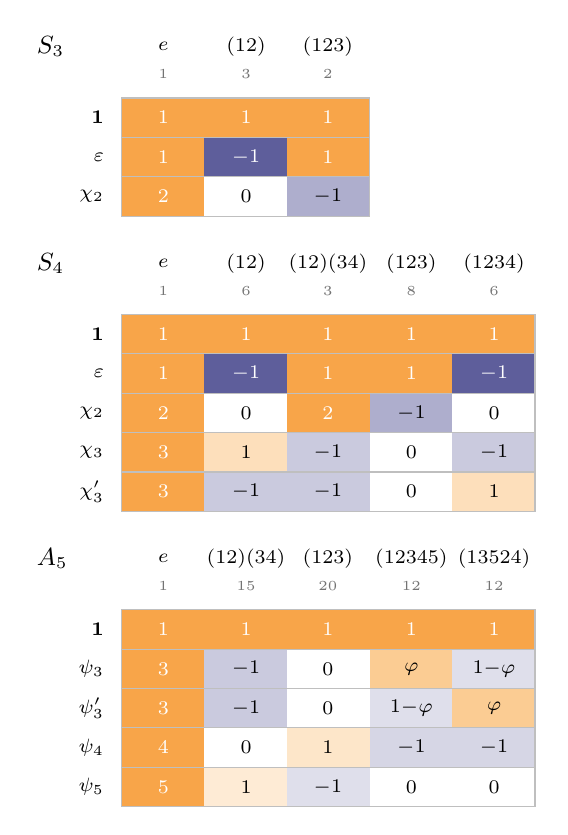
\begin{tikzpicture}[font=\scriptsize]
\node[anchor=west,font=\small] at (-1.2,0.55) {$\mathfrak S_3$};
\node at (0.53,0.55) {$e$};
\node[black!55,font=\tiny] at (0.53,0.2) {1};
\node at (1.58,0.55) {$(12)$};
\node[black!55,font=\tiny] at (1.58,0.2) {3};
\node at (2.62,0.55) {$(123)$};
\node[black!55,font=\tiny] at (2.62,0.2) {2};
\node[anchor=east] at (-0.1,-0.35) {$\mathbf 1$};
\fill[BurntOrange!70] (0.00,-0.60) rectangle (1.05,-0.10);
\node[text=white] at (0.53,-0.35) {$1$};
\fill[BurntOrange!70] (1.05,-0.60) rectangle (2.10,-0.10);
\node[text=white] at (1.58,-0.35) {$1$};
\fill[BurntOrange!70] (2.10,-0.60) rectangle (3.15,-0.10);
\node[text=white] at (2.62,-0.35) {$1$};
\draw[black!25] (0,-0.60) rectangle (3.15,-0.10);
\node[anchor=east] at (-0.1,-0.85) {$\varepsilon$};
\fill[BurntOrange!70] (0.00,-1.10) rectangle (1.05,-0.60);
\node[text=white] at (0.53,-0.85) {$1$};
\fill[MidnightBlue!70] (1.05,-1.10) rectangle (2.10,-0.60);
\node[text=white] at (1.58,-0.85) {$-1$};
\fill[BurntOrange!70] (2.10,-1.10) rectangle (3.15,-0.60);
\node[text=white] at (2.62,-0.85) {$1$};
\draw[black!25] (0,-1.10) rectangle (3.15,-0.60);
\node[anchor=east] at (-0.1,-1.35) {$\chi_2$};
\fill[BurntOrange!70] (0.00,-1.60) rectangle (1.05,-1.10);
\node[text=white] at (0.53,-1.35) {$2$};
\fill[white] (1.05,-1.60) rectangle (2.10,-1.10);
\node[text=black] at (1.58,-1.35) {$0$};
\fill[MidnightBlue!35] (2.10,-1.60) rectangle (3.15,-1.10);
\node[text=black] at (2.62,-1.35) {$-1$};
\draw[black!25] (0,-1.60) rectangle (3.15,-1.10);
\node[anchor=west,font=\small] at (-1.2,-2.2) {$\mathfrak S_4$};
\node at (0.53,-2.2) {$e$};
\node[black!55,font=\tiny] at (0.53,-2.55) {1};
\node at (1.58,-2.2) {$(12)$};
\node[black!55,font=\tiny] at (1.58,-2.55) {6};
\node at (2.62,-2.2) {$(12)(34)$};
\node[black!55,font=\tiny] at (2.62,-2.55) {3};
\node at (3.68,-2.2) {$(123)$};
\node[black!55,font=\tiny] at (3.68,-2.55) {8};
\node at (4.73,-2.2) {$(1234)$};
\node[black!55,font=\tiny] at (4.73,-2.55) {6};
\node[anchor=east] at (-0.1,-3.10) {$\mathbf 1$};
\fill[BurntOrange!70] (0.00,-3.35) rectangle (1.05,-2.85);
\node[text=white] at (0.53,-3.10) {$1$};
\fill[BurntOrange!70] (1.05,-3.35) rectangle (2.10,-2.85);
\node[text=white] at (1.58,-3.10) {$1$};
\fill[BurntOrange!70] (2.10,-3.35) rectangle (3.15,-2.85);
\node[text=white] at (2.62,-3.10) {$1$};
\fill[BurntOrange!70] (3.15,-3.35) rectangle (4.20,-2.85);
\node[text=white] at (3.68,-3.10) {$1$};
\fill[BurntOrange!70] (4.20,-3.35) rectangle (5.25,-2.85);
\node[text=white] at (4.73,-3.10) {$1$};
\draw[black!25] (0,-3.35) rectangle (5.25,-2.85);
\node[anchor=east] at (-0.1,-3.60) {$\varepsilon$};
\fill[BurntOrange!70] (0.00,-3.85) rectangle (1.05,-3.35);
\node[text=white] at (0.53,-3.60) {$1$};
\fill[MidnightBlue!70] (1.05,-3.85) rectangle (2.10,-3.35);
\node[text=white] at (1.58,-3.60) {$-1$};
\fill[BurntOrange!70] (2.10,-3.85) rectangle (3.15,-3.35);
\node[text=white] at (2.62,-3.60) {$1$};
\fill[BurntOrange!70] (3.15,-3.85) rectangle (4.20,-3.35);
\node[text=white] at (3.68,-3.60) {$1$};
\fill[MidnightBlue!70] (4.20,-3.85) rectangle (5.25,-3.35);
\node[text=white] at (4.73,-3.60) {$-1$};
\draw[black!25] (0,-3.85) rectangle (5.25,-3.35);
\node[anchor=east] at (-0.1,-4.10) {$\chi_2$};
\fill[BurntOrange!70] (0.00,-4.35) rectangle (1.05,-3.85);
\node[text=white] at (0.53,-4.10) {$2$};
\fill[white] (1.05,-4.35) rectangle (2.10,-3.85);
\node[text=black] at (1.58,-4.10) {$0$};
\fill[BurntOrange!70] (2.10,-4.35) rectangle (3.15,-3.85);
\node[text=white] at (2.62,-4.10) {$2$};
\fill[MidnightBlue!35] (3.15,-4.35) rectangle (4.20,-3.85);
\node[text=black] at (3.68,-4.10) {$-1$};
\fill[white] (4.20,-4.35) rectangle (5.25,-3.85);
\node[text=black] at (4.73,-4.10) {$0$};
\draw[black!25] (0,-4.35) rectangle (5.25,-3.85);
\node[anchor=east] at (-0.1,-4.60) {$\chi_3$};
\fill[BurntOrange!70] (0.00,-4.85) rectangle (1.05,-4.35);
\node[text=white] at (0.53,-4.60) {$3$};
\fill[BurntOrange!23] (1.05,-4.85) rectangle (2.10,-4.35);
\node[text=black] at (1.58,-4.60) {$1$};
\fill[MidnightBlue!23] (2.10,-4.85) rectangle (3.15,-4.35);
\node[text=black] at (2.62,-4.60) {$-1$};
\fill[white] (3.15,-4.85) rectangle (4.20,-4.35);
\node[text=black] at (3.68,-4.60) {$0$};
\fill[MidnightBlue!23] (4.20,-4.85) rectangle (5.25,-4.35);
\node[text=black] at (4.73,-4.60) {$-1$};
\draw[black!25] (0,-4.85) rectangle (5.25,-4.35);
\node[anchor=east] at (-0.1,-5.10) {$\chi_3'$};
\fill[BurntOrange!70] (0.00,-5.35) rectangle (1.05,-4.85);
\node[text=white] at (0.53,-5.10) {$3$};
\fill[MidnightBlue!23] (1.05,-5.35) rectangle (2.10,-4.85);
\node[text=black] at (1.58,-5.10) {$-1$};
\fill[MidnightBlue!23] (2.10,-5.35) rectangle (3.15,-4.85);
\node[text=black] at (2.62,-5.10) {$-1$};
\fill[white] (3.15,-5.35) rectangle (4.20,-4.85);
\node[text=black] at (3.68,-5.10) {$0$};
\fill[BurntOrange!23] (4.20,-5.35) rectangle (5.25,-4.85);
\node[text=black] at (4.73,-5.10) {$1$};
\draw[black!25] (0,-5.35) rectangle (5.25,-4.85);
\node[anchor=west,font=\small] at (-1.2,-5.95) {$A_5$};
\node at (0.53,-5.95) {$e$};
\node[black!55,font=\tiny] at (0.53,-6.3) {1};
\node at (1.58,-5.95) {$(12)(34)$};
\node[black!55,font=\tiny] at (1.58,-6.3) {15};
\node at (2.62,-5.95) {$(123)$};
\node[black!55,font=\tiny] at (2.62,-6.3) {20};
\node at (3.68,-5.95) {$(12345)$};
\node[black!55,font=\tiny] at (3.68,-6.3) {12};
\node at (4.73,-5.95) {$(13524)$};
\node[black!55,font=\tiny] at (4.73,-6.3) {12};
\node[anchor=east] at (-0.1,-6.85) {$\mathbf 1$};
\fill[BurntOrange!70] (0.00,-7.10) rectangle (1.05,-6.60);
\node[text=white] at (0.53,-6.85) {$1$};
\fill[BurntOrange!70] (1.05,-7.10) rectangle (2.10,-6.60);
\node[text=white] at (1.58,-6.85) {$1$};
\fill[BurntOrange!70] (2.10,-7.10) rectangle (3.15,-6.60);
\node[text=white] at (2.62,-6.85) {$1$};
\fill[BurntOrange!70] (3.15,-7.10) rectangle (4.20,-6.60);
\node[text=white] at (3.68,-6.85) {$1$};
\fill[BurntOrange!70] (4.20,-7.10) rectangle (5.25,-6.60);
\node[text=white] at (4.73,-6.85) {$1$};
\draw[black!25] (0,-7.10) rectangle (5.25,-6.60);
\node[anchor=east] at (-0.1,-7.35) {$\psi_3$};
\fill[BurntOrange!70] (0.00,-7.60) rectangle (1.05,-7.10);
\node[text=white] at (0.53,-7.35) {$3$};
\fill[MidnightBlue!23] (1.05,-7.60) rectangle (2.10,-7.10);
\node[text=black] at (1.58,-7.35) {$-1$};
\fill[white] (2.10,-7.60) rectangle (3.15,-7.10);
\node[text=black] at (2.62,-7.35) {$0$};
\fill[BurntOrange!38] (3.15,-7.60) rectangle (4.20,-7.10);
\node[text=black] at (3.68,-7.35) {$\varphi$};
\fill[MidnightBlue!14] (4.20,-7.60) rectangle (5.25,-7.10);
\node[text=black] at (4.73,-7.35) {$1{-}\varphi$};
\draw[black!25] (0,-7.60) rectangle (5.25,-7.10);
\node[anchor=east] at (-0.1,-7.85) {$\psi_3'$};
\fill[BurntOrange!70] (0.00,-8.10) rectangle (1.05,-7.60);
\node[text=white] at (0.53,-7.85) {$3$};
\fill[MidnightBlue!23] (1.05,-8.10) rectangle (2.10,-7.60);
\node[text=black] at (1.58,-7.85) {$-1$};
\fill[white] (2.10,-8.10) rectangle (3.15,-7.60);
\node[text=black] at (2.62,-7.85) {$0$};
\fill[MidnightBlue!14] (3.15,-8.10) rectangle (4.20,-7.60);
\node[text=black] at (3.68,-7.85) {$1{-}\varphi$};
\fill[BurntOrange!38] (4.20,-8.10) rectangle (5.25,-7.60);
\node[text=black] at (4.73,-7.85) {$\varphi$};
\draw[black!25] (0,-8.10) rectangle (5.25,-7.60);
\node[anchor=east] at (-0.1,-8.35) {$\psi_4$};
\fill[BurntOrange!70] (0.00,-8.60) rectangle (1.05,-8.10);
\node[text=white] at (0.53,-8.35) {$4$};
\fill[white] (1.05,-8.60) rectangle (2.10,-8.10);
\node[text=black] at (1.58,-8.35) {$0$};
\fill[BurntOrange!18] (2.10,-8.60) rectangle (3.15,-8.10);
\node[text=black] at (2.62,-8.35) {$1$};
\fill[MidnightBlue!18] (3.15,-8.60) rectangle (4.20,-8.10);
\node[text=black] at (3.68,-8.35) {$-1$};
\fill[MidnightBlue!18] (4.20,-8.60) rectangle (5.25,-8.10);
\node[text=black] at (4.73,-8.35) {$-1$};
\draw[black!25] (0,-8.60) rectangle (5.25,-8.10);
\node[anchor=east] at (-0.1,-8.85) {$\psi_5$};
\fill[BurntOrange!70] (0.00,-9.10) rectangle (1.05,-8.60);
\node[text=white] at (0.53,-8.85) {$5$};
\fill[BurntOrange!14] (1.05,-9.10) rectangle (2.10,-8.60);
\node[text=black] at (1.58,-8.85) {$1$};
\fill[MidnightBlue!14] (2.10,-9.10) rectangle (3.15,-8.60);
\node[text=black] at (2.62,-8.85) {$-1$};
\fill[white] (3.15,-9.10) rectangle (4.20,-8.60);
\node[text=black] at (3.68,-8.85) {$0$};
\fill[white] (4.20,-9.10) rectangle (5.25,-8.60);
\node[text=black] at (4.73,-8.85) {$0$};
\draw[black!25] (0,-9.10) rectangle (5.25,-8.60);
\end{tikzpicture}
